\documentclass[11pt]{scrartcl}
\usepackage{dominatrix}
\usepackage{colortbl}
\usepackage{pgfplots}
\newcommand{\jon}{J\'{o}n }
\newcommand{\oneth}{\ensuremath{\frac{1}{3}}}
\newcommand{\twoth}{\ensuremath{\frac{2}{3}}}
\newcommand{\ve}{\varepsilon}
\pgfplotsset{compat=1.9}
\definecolor{light-gray}{gray}{0.75}
\title{Midterm Review Session}
\subject{ECON W3213 Spring 2014 \jon Steinsson}
\author{Linan Qiu, lq2137}
\begin{document}

\maketitle

\begin{abstract}
This is a set of questions to get you \textbf{started} on revision. They are very very basic. Don't expect the midterm to be this easy (just check out the sample midterm!) Don't be too happy if you can answer these. After all, these are the \textbf{bare basics}. If you can't answer them, however, you're in deep shit. In that case, as Gandalf says, you shall not pass.
\end{abstract}

\section{Production}

This is the Cobb-Douglas production function

\[Y = \bar{A}K^\alpha L^{\beta} \]

\begin{enumerate}
\item If $\beta = 1- \alpha$ and $0 < \alpha < 1$
\begin{enumerate}
\item Show that the production function is increasing in both $K$ and $L$
\item Show that it exhibits diminishing returns to $K$ and diminishing returns to $L$
\item Show that it exhibits constant returns to scale
\end{enumerate}
\item If $\alpha > 1$ and $\beta > 1$
\begin{enumerate}
\item Show that it is increasing in both $K$ and $L$
\item Show that it does not exhibit diminishing returns to either $K$ or $L$
\item Show that it exhibits increasing returns to scale
\end{enumerate}
\item For a firm,
\begin{enumerate}
\item What is the cost of capital?
\item What is the cost of labor?
\item What is the firm's profit?
\item How does a firm optimize capital input?
\item How does a firm optimize labor input?
\item What share of output goes to workers?
\item What share of output goes to capital?
\end{enumerate}
\item What is the output $y = \frac{Y}{L}$ in per capita terms?
\end{enumerate}

\section{Household Behavior}

Your overall utility is 

\[U(C) - V(H)\]

\begin{enumerate}
\item Given that you love consuming and you hate working,
\begin{enumerate}
\item What does $U$ represent?
\item What does $V$ represent?
\end{enumerate}
\item For $U(C)$
\begin{enumerate}
\item What is the sign of $U'(C) = \frac{\partial U(C)}{\partial C}$?
\item What is the sign of $U''(C) = \frac{\partial^2 U(C)}{\partial C^2}$?
\item Plot $U(C)$ agains $C$
\end{enumerate}
\item For $V(H)$
\begin{enumerate}
\item What is the sign of $V'(H)$?
\item What is the sign of $V''(H)$?
\item Plot $V(H)$ against $H$
\end{enumerate}
\end{enumerate}

You can only consume what you earn, hence

\[ C = wH\]

\begin{enumerate}
\item Labor Supply using Constrained Optimization
\begin{enumerate}
\item Express $U(C)$ as a function of $w$ and $H$
\item How does one maximize utility given the budget constraint?
\item What is the labor supply equation?
\end{enumerate}
\item Labor Supply using Calculus of Variations
\begin{enumerate}
\item Derive the labor supply equation using calculus of variations
\end{enumerate}
\item Labor Demand
\begin{enumerate}
\item What is the labor demand equation?
\end{enumerate}
\item Substitution Effect
\begin{enumerate}
\item Without changing consumption $C$, what happens when wages $w$ increase?
\item When wages $w$ decrease?
\end{enumerate}
\item Income Effect
\begin{enumerate}
\item Without changing wages $w$, what happens when consumption $C$ increases?
\item When consumption $C$ decreases?
\end{enumerate}
\item Taxation
\begin{enumerate}
\item Does the utility function change due to taxation?
\item How does the budget constraint change when we consider income tax, consumption tax, and government transfers?
\item Find the equilibrium wage
\item Is this higher than or lower than the tax free wage?
\end{enumerate}
\item Now let's use specific functional forms. $U(C) = \log{C}$ and $V(H) = \psi \frac{H^{1+\eta}}{1+\eta}$
\begin{enumerate}
\item Prove that these forms for $U(C)$ and $V(H)$ produces the signs that we want for $U'(C)$ $U''(C)$ $V'(H)$ and $V''(H)$
\item What is labor demand equation in this specific case?
\item What is the labor supply equation in this specific case?
\item Take the log of the equilibrium. What conclusions can we get regarding percentage change in hours of labor?
\item What is the Frisch elasticity of labor supply?
\end{enumerate}
\end{enumerate}

\section{Market Efficiency}
\begin{enumerate}
\item Pareto Efficiency
\begin{enumerate}
\item Define pareto efficiency in your own words
\item What are the 3 forms of efficiency that we need for pareto efficiency?
\end{enumerate}
\item Exchange Efficiency
\begin{enumerate}
\item Derive the condition that guarantees exchange efficiency
\item Express this on an edgeworth box and show the set of points that are exchange efficient
\item Convince yourself that this should also apply to all other pairs of outputs
\end{enumerate}
\item Production Efficiency
\begin{enumerate}
\item Derive the condition that guarantees production efficiency
\item Convince yourself that this should also apply to all other pairs of inputs
\end{enumerate}
\item Land Efficiency
\begin{enumerate}
\item Derive the condition that guarantees land efficiency
\item Convince yourself that this should also apply to all other pairs of input and land
\end{enumerate}
\item Prices
\begin{enumerate}
\item How do prices ensure efficiency in each of these markets
\end{enumerate}
\item Market Failure
\begin{enumerate}
\item In your own words, explain 5 types of market failure using examples
\end{enumerate}
\end{enumerate}

\section{Consumption Savings}

Your utility function is

\[U(C_1) + \beta U(C_2)\]

Your budget function is 

\[C_1 + B = Y_1\]

\[C_2 = Y_2 + (1+R)B\]

\begin{enumerate}
\item Using the utility function above
\begin{enumerate}
\item Explain what $\beta$ is
\end{enumerate}
\item Using the budget function
\begin{enumerate}
\item What are the lower and upper limits for B?
\item Combine them into a single equation without B
\item Explain intuitively what that equation means using the concept of present value
\end{enumerate}
\item To derive the Consumption Euler Equation,
\begin{enumerate}
\item Express $C_2$ in terms of $C_1$
\item Maximize utility subject to the budget constraint
\item Derive the Consumption Euler Equation
\end{enumerate}
\item If $U(C) = \log{C}$
\begin{enumerate}
\item Show that this function is increasing and exhibits diminishing marginal utility
\item Derive the consumption euler equation for this specific functional form
\end{enumerate}
\item Using the Consumption Euler Equation,
\begin{enumerate}
\item Show that level of consumption does not depend on level of period specific income, only total income
\item Level of consumption is a fraction of the present value of income. Find that fraction.
\end{enumerate}
\item Extend what we have so far to 3 periods and derive the same two conclusions
\item Generalize this to $n$ periods and show that the two conclusions still remain true

\begin{figure}[H]
\begin{subfigure}[b]{0.5\textwidth}
\centering
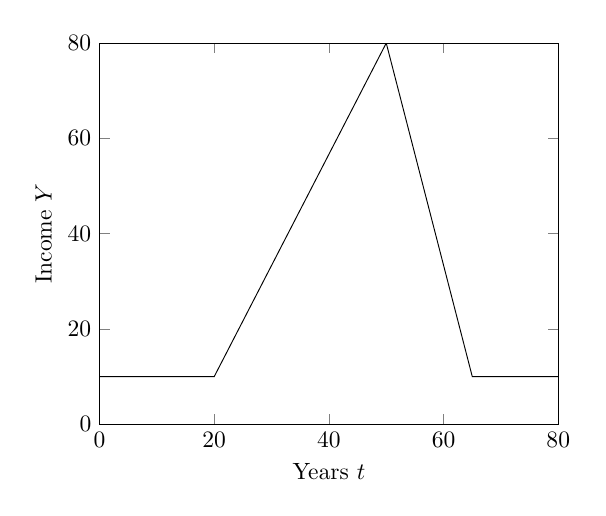
\begin{tikzpicture}[scale=0.85]
\begin{axis}[ylabel = {Income $Y$}, xlabel = {Years $t$}, xmin = 0, xmax = 80,ymin = 0, ymax = 80]

\addplot[black, domain=0:80]
coordinates{(0,10) (20,10) (50, 80) (65,10) (80,10)};

\end{axis}
\end{tikzpicture}
\end{subfigure}
\hspace{2ex}
\begin{subfigure}[b]{0.5\textwidth}
\centering
\begin{tikzpicture}[scale=0.85]
\begin{axis}[ylabel = {Consumption $C$}, xlabel = {Years $t$}, xmin = 0, xmax = 80,ymin = 0, ymax = 80]

\addplot[blue, domain=0:80]
coordinates{(0,26.875) (80, 26.875)};

\end{axis}
\end{tikzpicture}
\end{subfigure}
\caption{Income and Consumption Level throughout Lifetime}
\end{figure}

\begin{figure}[H]
\centering
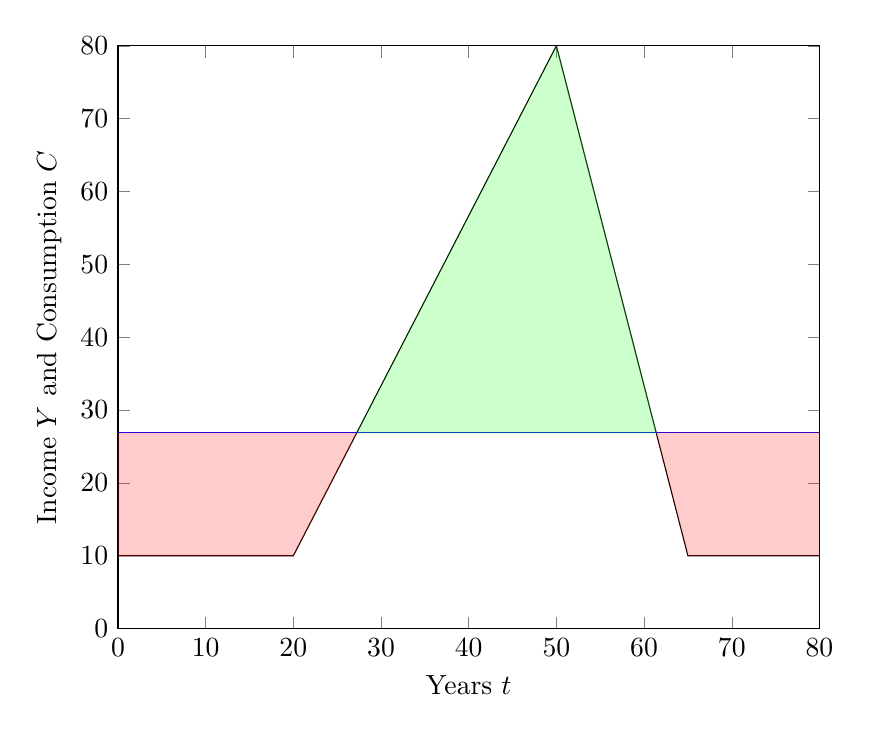
\begin{tikzpicture}
\begin{axis}[ylabel = {Income $Y$ and Consumption $C$}, xlabel = {Years $t$}, xmin = 0, xmax = 80,ymin = 0, ymax = 80, scale=1.3]

\addplot[black, domain=0:80]
coordinates{(0,10) (20,10) (50, 80) (65,10) (80,10)};

\addplot[blue, domain=0:80]
coordinates{(0,26.875) (80, 26.875)};

\addplot[fill, red, opacity = 0.2]
coordinates{(0,10) (20,10) (27.2322,26.875) (0, 26.875)};

\addplot[fill, red, opacity = 0.2]
coordinates{(65,10) (80,10) (80,26.875) (61.3839, 26.875)} ;

\addplot[fill, green, opacity = 0.2]
coordinates{(27.2322,26.875) (61.3839, 26.875) (50,80)};

\addplot[black, domain=0:80]
coordinates{(0,0)};

\end{axis}
\end{tikzpicture}
\caption{Borrowing, Saving and Dissavings}
\end{figure}

\item Referring to the graphs above
\begin{enumerate}
\item When is a person borrowing, saving, and dissaving? 
\item Why is the consumption line a straight line?
\item Which of the shaded areas are equal to which others?
\end{enumerate}
\end{enumerate}

\section{Malthus Growth Model}

The production function is

\[Y_t = A_t D^\alpha L_t^{1-\alpha} \]

\begin{enumerate}
\item $0 < \alpha < 1$. Convince yourself that this function exhibits
\begin{enumerate}
\item Constant returns to scale
\item Diminishing returns to labor
\end{enumerate}
\item Labor Demand and Supply
\begin{enumerate}
\item Derive the labor demand equation
\item State the labor supply equation
\item Find the equilibrium wage
\end{enumerate}

The Malthus Population Growth Equation is given by 

\[ \frac{N_{t+1}}{N_t} = \left(\frac{w_t}{w_s}\right)^\gamma \xi_t \]

\item What is
\begin{enumerate}
\item $w_s$
\item $\gamma$
\item $\xi_t$ and what is the value that $\xi_t$ should take under normal circumstances?
\end{enumerate}
\item Express $N_{t+1}$ in terms of $N_t$ and graph that.
\item Explain how population changes if $N_t < N_{t+1}$ or $N_t > N_{t+1}$
\item Find the steady state population
\item What happens to wages at the steady state population? It is higher than or lower than the subsistence wage $w_s$?
\item How will shocks affect both population and wages in the short run and long run if
\begin{enumerate}
\item The shock was a temporary disease that decreased population
\item The shock was a permanent increase in technology
\item For both of the above, illustrate what happens to population and wages in the short run and long run on two graphs -- one for population and the other for wages
\end{enumerate}
\end{enumerate}

\section{Solow-Swan Growth Model}

The production function is

\[ Y = \bar{A}K^{\oneth}L^{\twoth} \]

\begin{enumerate}
\item Convince yourself that this function exhibits
\begin{enumerate}
\item Constant returns to scale
\item Diminishing returns to labor
\item Diminishing returns to labor
\end{enumerate}
\item Given that $s$ of $Y$ is saved, find investments
\item Find consumption
\item To find the steady state capital,
\begin{enumerate}
\item What is the inflow of capital for every period?
\item What is the outflow of capital for every period?
\item Derive the steady state capital
\item Graph $dK$, $I$, and $Y$ on the same graph, showing the steady state and consumption at the steady state
\item What happens if the starting stock of capital is below the steady state? What about above?
\end{enumerate}
\item How will shocks affect both capital and income in the short run and long run if
\begin{enumerate}
\item The shock is a temporary increase in capital (perhaps foreign aid?)
\item The shock is a permanent increase in technology $\bar{A}$
\item The shock is a permanent increase in $d$ depreciation
\end{enumerate}
\item Do 2, 3, 4, and 5 for the Solow-Swan model with Labor Changes where $L_{t+1} = L_t (1+\bar{n})$
\item Is unconditional convergence empirically true? Is conditional convergence empirically true? Explain.
\end{enumerate}




\end{document}